The earliest learnings from the experiments have shown presented that the severe class imbalance is present and the model tends to predict mostly pure background. In order to overcome this one can use an asymmetrical loss during training. Similarily to a weighted loss for a classification problem wihth class imbalance, a weigted loss for segmentation task can be introduced. In this case different pixels of the prediction will recieve a different weight based on some criteria. Yet the use of weights cannot be easily defined for a Pearson correlation coefficients, it is possible to apply it to MSE loss function as the coefficients there can be added directly in front of the squared difference between pixels. 
\begin{figure}[H]
	\begin{center}
		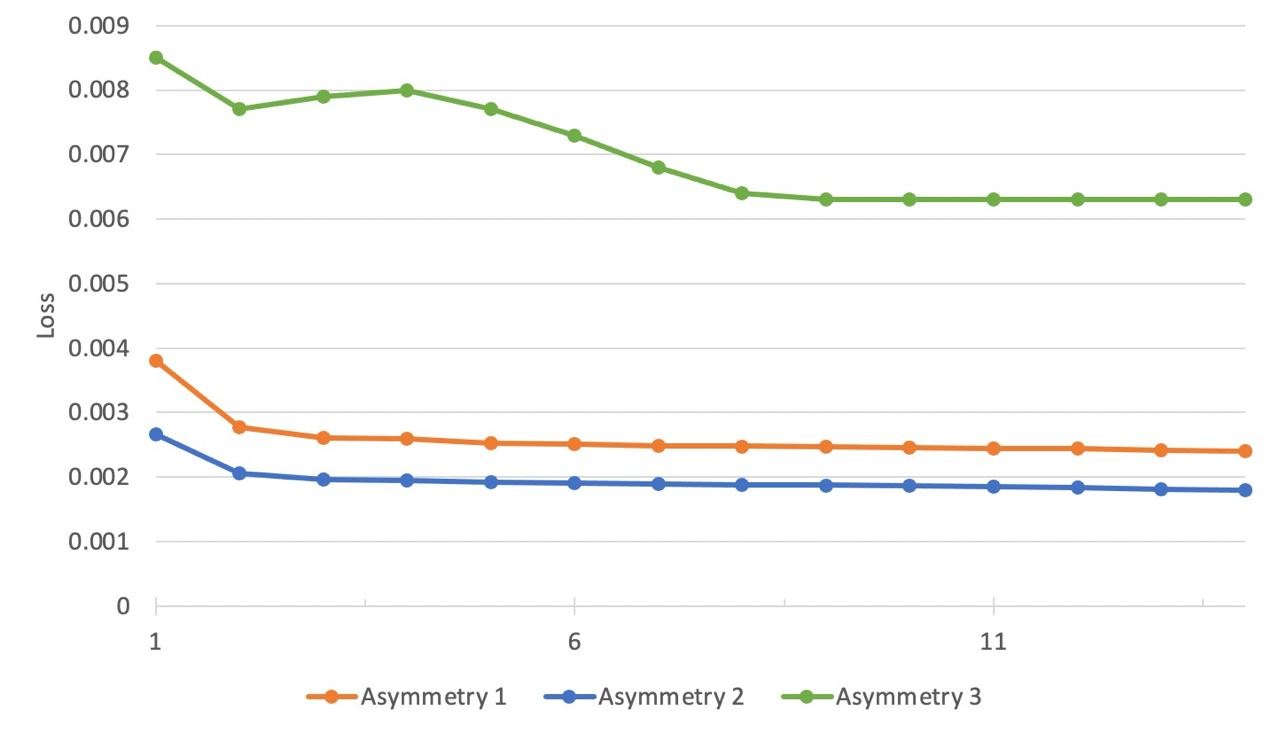
\includegraphics[width=0.5\linewidth]{bilder/golgi/asymmetrical-training.jpg}
		\caption{Punishing over and under predictions with asymmetrical MSE loss}\label{fig:golgi-asymmetrical-training}
	\end{center}
\end{figure}

In Figure \ref{fig:golgi-asymmetrical-training} are presented training learning curves from three asymmetrical approaches: 
\begin{figure}[H]
	\begin{center}
		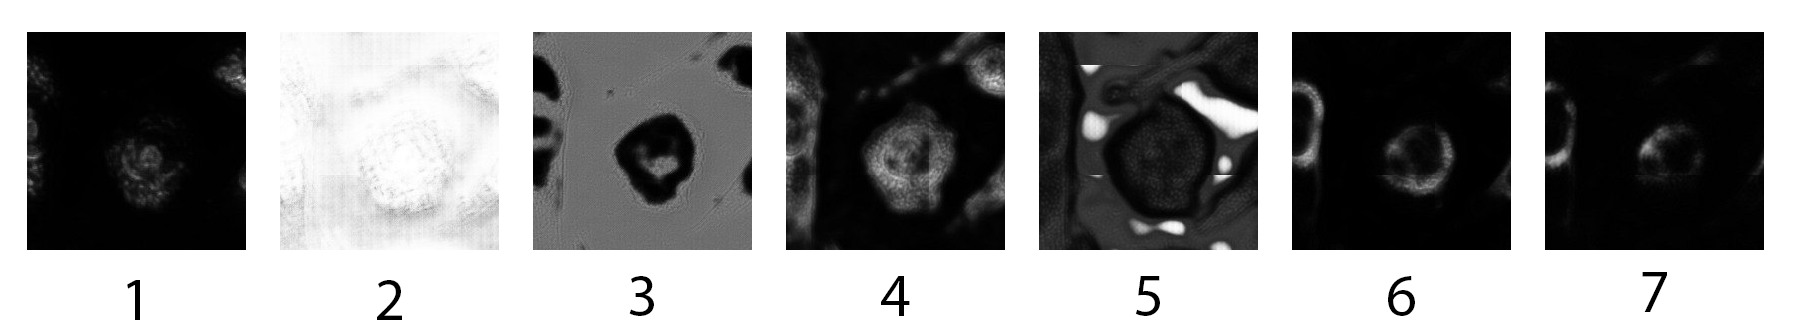
\includegraphics[width=\linewidth]{bilder/golgi/asymmetrical-predictions.png}
		\caption{Results of advanced versions of MSE training}\label{fig:golgi-asymmetrical-predictions}
	\end{center}
\end{figure} 

Asymmetry 1 is aimed to punish an underprediction: when a models pixel prediction is lower than a true one the loss will be higher.
\begin{lstlisting}
	residual = prediction - ground_truth
	loss = torch.where(residual > 0, residual ** 2, 2 * (residual) ** 2)
	loss = torch.mean(loss)
  \end{lstlisting}

Asymmetry 2 is a reverse of Asymmetry 1 and is aimed to punish an overprediction: when a models pixel prediction is higher than a true one the loss will be higher.
  \begin{lstlisting}
	  residual = prediction - ground_truth
	  loss = torch.where(residual < 0, residual ** 2, 2 * (residual) ** 2)
	  loss = torch.mean(loss)
	\end{lstlisting}

Asymmetry 3 is a stronger version of Asymmetry 1 and is aimed to punish an underprediction $10$ times stronger.
	\begin{lstlisting}
		residual = prediction - ground_truth
		loss = torch.where(residual > 0, residual ** 2, 10 * (residual) ** 2)
		loss = torch.mean(loss)
	  \end{lstlisting}

All of the approaches above do not bring a big change in the performance and a mostly black image remained to be an output. Interestingly, punishing underprediction has essentially backfired, as loss then supports an overprediction. Because setting the weights of one class to be smaller is the same as setting the weights of the other class to be larger, and here as a result the model is more likely to overpredict. That is why the second asymmetry has a better loss, even though the logic behind it is not that obvious at first. 

There were other interesting approaches in asymmetrical losses tested that are depicted in Figure \ref{fig:golgi-asymmetrical-training}

1. Adjusting overall brightness. Leads the an absence of bright spots in the prediction and an absence of brightness gradients.
\begin{lstlisting}
	loss = loss +  prediction.sum() / ground_truth.sum()
  \end{lstlisting}

2. Adjusting overall brightness with a reversed division. Leads to fully white images as this would minimize the fraction in loss.
\begin{lstlisting}
	loss = loss + ground_truth.sum() / prediction.sum()
\end{lstlisting}

3. Combining asymmetry from multiplication with prediction with overall brightness

\begin{lstlisting}
	loss = MSE(ground_truth, prediction)
	loss = torch.mul(loss, prediction.abs()) + ground_truth.sum() / prediction.sum()
\end{lstlisting}

4.
\begin{lstlisting}
	loss = MSE(ground_truth, prediction)
	loss = torch.mul(loss, (1 - ground_truth).abs()) + ground_truth.sum() / prediction.sum()
\end{lstlisting}

5.
\begin{lstlisting}
	loss = MSE(ground_truth, prediction)
	loss = torch.mul(loss, ground_truth.abs()) + ground_truth.sum() / prediction.sum()
\end{lstlisting}

6. Usual MSE

7. Usual PCC